\section{Datacenter structure}

In a typical data center building, only about half of the available space is used for actual servers. 
The remaining space is dedicated to cooling systems and energy management.
\begin{figure}[H]
    \centering
    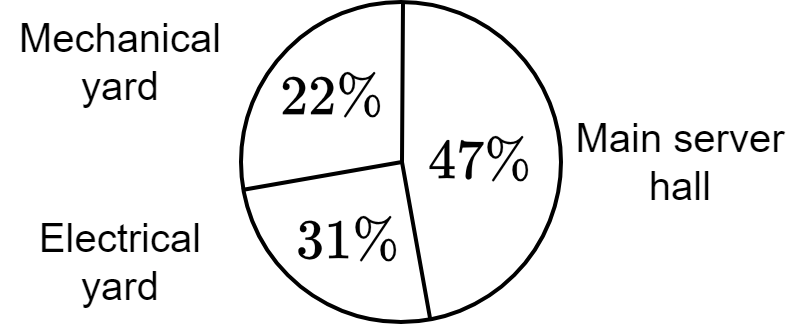
\includegraphics[width=0.5\linewidth]{images/build.png}
    \caption{Usual building usage}
\end{figure}
A WSC includes critical components beyond servers, such as power delivery systems, cooling infrastructure, and building facilities, all of which are essential for its operation.

\subsection{Power system}
To protect against power failures, data centers use battery systems and diesel generators to back up the external power supply. 
A typical Uninterruptible Power Supply (UPS) integrates three functions: energy storage, switch for active power input, and elimination of voltage spikes. 

Data center power consumption can reach several megawatts, with cooling systems typically consuming about half of the total energy used by IT equipment (servers, network infrastructure, and storage). 
Globally, data centers account for approximately 3\% of the world's electricity supply and contribute about 2\% of total greenhouse gas emissions. 
This highlights the urgent need for energy-efficient solutions and sustainable practices in the data center industry.

\paragraph*{Power usage effectiveness}
Power Usage Effectiveness (PUE) measures the energy efficiency of a data center:
\[\text{PUE}=\dfrac{\text{Total facility power}}{\text{IT equipment power}}\]
Total facility power includes the energy consumption of IT systems (servers, network devices, storage units) and other equipment like cooling systems, UPS, switchgear, generators, lighting, and fans. 
Data Center Infrastructure Efficiency (DCIE) is the reciprocal of PUE.

\subsection{Cooling systems}
IT equipment generates substantial heat, requiring an expensive and efficient cooling system. 
This system typically includes coolers, heat exchangers, and cold water tanks. 
The main cooling system types are:
\begin{itemize}
    \item \textit{Open loop}: utilizes cold outside air to produce chilled water or directly cool servers. 
        It is cost-effective compared to traditional chillers.
    \item \textit{Closed loop}: common on the data center floor, this system extracts and expels heat from servers, directing it to a heat exchanger. 
        Cooled air is then recirculated to the servers.
    \item \textit{Two loop}: involves primary and secondary loops. 
        The primary loop includes airflow from the underfloor plenum, through the racks, and back to the Computer Room Air Conditioning (CRAC) unit. 
        The secondary loop circulates liquid coolant from the CRAC to external heat exchangers, which release heat into the environment.
    \item \textit{Three loop}: involves primary air circuit, secondary liquid cooling loop, and tertiary heat rejection loop. 
        This setup manages the thermal environment effectively.
\end{itemize}
A water-cooled chiller operates similarly to a water-cooled air conditioner, using cooling towers to cool a water stream by evaporating a portion into the atmosphere. 
In-rack and in-row coolers place air-to-water heat exchangers near the servers to shorten the distance for heat dissipation.

Direct cooling of server components can be achieved with cold plates, which are liquid-cooled heat sinks. 
These are used for components with the highest power dissipation, while other components rely on air cooling. 
The liquid carries heat to a liquid-to-air or liquid-to-liquid heat exchanger, which can be located near the tray or rack, or integrated into the data center infrastructure, such as a cooling tower.

\subsection{Datacenter taxonomy}
Datacenter availability is categorized into four distinct tier levels, each with specific requirements:
\begin{table}[H]
    \centering
    \begin{tabular}{|c|l|}
    \hline
    Tier level & \multicolumn{1}{c|}{Requirements} \\ \hline
    1          & \makecell[l]{No redundancy \\ 99.671\% uptime per year \\ Maximum of 28.8 hours of downtime per year }                                 \\\hline
    2          & \makecell[l]{Some cooling and power redundancies \\ 99.741\% uptime per year \\ No more than 22 hours of downtime per year}    \\\hline
    3          & \makecell[l]{$N+1$ fault tolerance \\ 99.982\% uptime \\ Less than 1.6 hours of downtime per year} \\\hline
    4          & \makecell[l]{$2N$ or $2N+1$ fault tolerance \\ 99.995\% uptime per year \\ Less than 26.3 minutes of downtime per year}                                 \\ \hline
    \end{tabular}
\end{table}